\PassOptionsToPackage{table}{xcolor}
\documentclass[10pt,aspectratio=169]{beamer}

\usetheme{metropolis}
\usepackage{appendixnumberbeamer}
\usepackage{booktabs}
\usepackage{array}
\usepackage{multirow}
\usepackage{tikz}
\usetikzlibrary{
  positioning,
  arrows.meta,
  decorations.pathmorphing,
  calc,
  fit,
  shapes.geometric,
  backgrounds,
  chains,
  matrix
}
\usepackage{amsmath,amssymb}
\usepackage{xcolor}

% --- Colors ---
\definecolor{accent}{HTML}{3498DB}
\definecolor{phoneme}{HTML}{E74C3C}
\definecolor{circuit}{HTML}{27AE60}
\definecolor{backbone}{HTML}{F39C12}
\definecolor{fusion}{HTML}{9B59B6}
\definecolor{chill}{HTML}{95A5A6}
\definecolor{tok}{HTML}{E67E22}

\setbeamercolor{alerted text}{fg=phoneme}

\hypersetup{
  colorlinks=true,
  linkcolor=.,
  urlcolor=accent,
  citecolor=accent
}

\title{Phonological Assembly Circuits in GPT-2}
\subtitle{How Transformers Compute Sound Structure from Orthography}
\author{Elliot Tower}
\date{}

\begin{document}

% =============================================
% TITLE
% =============================================
\begin{frame}[plain]
\maketitle
\end{frame}

% =============================================
% OVERVIEW
% =============================================
\begin{frame}{Overview}
\hypertarget{sl:overview}{}

\begin{columns}[T]
\begin{column}{0.48\textwidth}
\textbf{Part 1: The Question}
\begin{enumerate}
  \item \hyperlink{sl:motivation}{Motivation}
  \item \hyperlink{sl:operations}{The six operations}
  \item \hyperlink{sl:oronym}{The oronym problem}
\end{enumerate}

\vspace{0.8em}
\textbf{Part 2: Methods}
\begin{enumerate}\setcounter{enumi}{3}
  \item \hyperlink{sl:datasets}{Datasets}
  \item \hyperlink{sl:discovery}{Circuit discovery}
\end{enumerate}
\end{column}

\begin{column}{0.48\textwidth}
\textbf{Part 3: Circuits}
\begin{enumerate}\setcounter{enumi}{5}
  \item \hyperlink{sl:backbone}{Backbone hypothesis}
  \item \hyperlink{sl:fusionheads}{Fusion heads}
  \item \hyperlink{sl:composition}{Compositional validation}
\end{enumerate}

\vspace{0.8em}
\textbf{Part 4: Implications}
\begin{enumerate}\setcounter{enumi}{8}
  \item \hyperlink{sl:tokenization}{Tokenization bottleneck}
  \item \hyperlink{sl:discussion}{Discussion}
\end{enumerate}
\end{column}
\end{columns}
\end{frame}

% =============================================
% PART 1 DIVIDER
% =============================================
\begin{frame}[plain,noframenumbering]
\begin{center}
\vfill
  \fcolorbox{black}{white}{\parbox{0.65\textwidth}{\centering\vspace{0.8em}
    {\Large\bfseries Part 1: The Question}
  \vspace{0.8em}}}
\vfill
\end{center}
\end{frame}

% =============================================
% MOTIVATION
% =============================================
\begin{frame}{Why phonological circuits?}
\hypertarget{sl:motivation}{}

The MI literature has characterized circuits for:
\begin{itemize}
  \item Syntax: IOI, subject--verb agreement, reflexive anaphora
  \item Retrieval: induction heads, greater-than
  \item Factual: capital cities, birth years
\end{itemize}

\vspace{0.8em}
\textbf{Gap:} zero circuit-level work on \alert{phonological} computation.

\vspace{0.8em}
Yet LLMs demonstrably encode sound structure:
\begin{itemize}
  \item Linear probes on GPT-2 mid-layers: 63--79\% rhyme detection (\href{https://aclanthology.org/2026.latechclfl-1.9}{Liao \& Shi, 2026})
  \item Above-chance grapheme-to-phoneme conversion (\href{https://arxiv.org/abs/2404.02456}{PhonologyBench, 2024})
\end{itemize}

\vspace{0.8em}
\textbf{Question:} \emph{Which attention heads compute phonological knowledge?}
\end{frame}

% =============================================
% THE PUZZLE
% =============================================
\begin{frame}{The puzzle}

BPE tokenization encodes \textbf{orthography}, not phonology.

\vspace{0.5em}
Yet the model can do this:

\vspace{0.8em}
\begin{center}
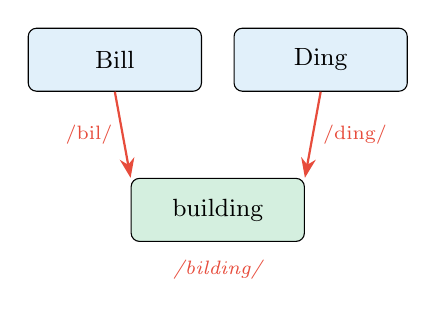
\begin{tikzpicture}[
  box/.style={draw, rounded corners=3pt, minimum height=0.8cm, minimum width=2.2cm, font=\small},
  arr/.style={-{Stealth[length=2.5mm]}, thick}
]
  \node[box, fill=accent!15] (bill) {Bill};
  \node[box, fill=accent!15, right=0.4cm of bill] (ding) {Ding};

  \node[box, fill=circuit!20, below=1.5cm of $(bill)!0.5!(ding)$] (building) {building};

  \draw[arr, phoneme] (bill.south) -- (building.north west) node[midway, left, font=\scriptsize] {/bil/};
  \draw[arr, phoneme] (ding.south) -- (building.north east) node[midway, right, font=\scriptsize] {/ding/};
  \node[below=0.1cm of building, font=\scriptsize\itshape, phoneme] {/bilding/};
\end{tikzpicture}
\end{center}

\vspace{0.5em}
\textbf{Cross-boundary phoneme fusion} from purely orthographic input.

How? Which heads? Is there a dedicated circuit?
\end{frame}

% =============================================
% THE SIX OPERATIONS
% =============================================
\begin{frame}{Six phonological operations}
\hypertarget{sl:operations}{}

\begin{center}
\small
\begin{tabular}{clllr}
\toprule
\textbf{Op} & \textbf{Linguistic term} & \textbf{Example} & \textbf{Computation} & \textbf{N} \\
\midrule
1 & Rhyming hypocorism & Richard $\to$ Dick & Irregular stored lookup & 32 \\
2 & Clipping (apocope) & Timothy $\to$ Tim & First-syllable truncation & 90 \\
3 & Initialism & J $\to$ Jay & Grapheme $\to$ phoneme name & 30 \\
4 & \textbf{Oronym} & \textbf{Bill Ding $\to$ building} & \textbf{Cross-boundary fusion} & \textbf{99} \\
5 & Homophone & Neil $\to$ kneel & Phoneme-identity detection & 120 \\
7 & Folk etymology & microwave $\to$ Michael Wave & Reverse decomposition & 75 \\
\bottomrule
\end{tabular}
\end{center}

\vspace{0.5em}
Each requires a \textbf{linguistically distinct} computation.

$\Rightarrow$ Predicts \textbf{distinct circuit architectures}.
\end{frame}

% =============================================
% OPERATIONS DIAGRAM
% =============================================
\begin{frame}{Operations as a computational taxonomy}

\begin{center}
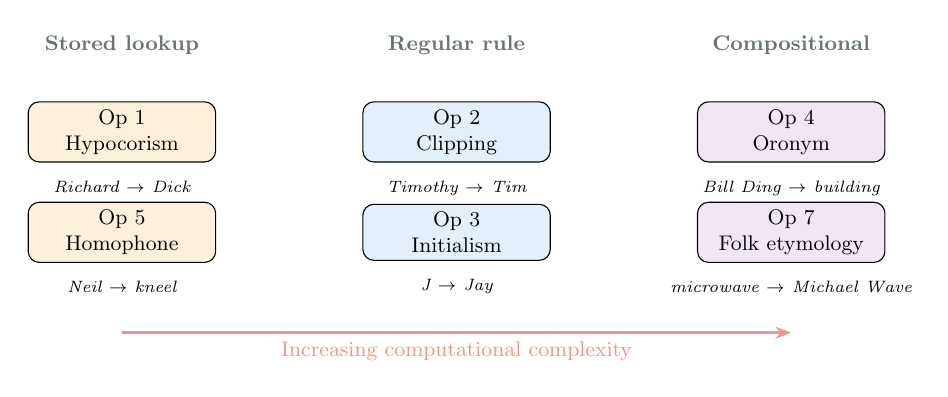
\begin{tikzpicture}[
  scale=0.85, transform shape,
  op/.style={draw, rounded corners=4pt, minimum height=0.7cm, minimum width=2.8cm,
             font=\small, align=center},
  cat/.style={draw=none, font=\small\bfseries, text=chill!70!black},
  arr/.style={-{Stealth[length=2mm]}, thick, chill}
]
  % Categories
  \node[cat] (stored) at (0, 2.5) {Stored lookup};
  \node[cat] (regular) at (5, 2.5) {Regular rule};
  \node[cat] (compositional) at (10, 2.5) {Compositional};

  % Operations
  \node[op, fill=backbone!15] (op1) at (0, 1.2) {Op 1\\Hypocorism};
  \node[op, fill=backbone!15] (op5) at (0, -0.3) {Op 5\\Homophone};

  \node[op, fill=accent!15] (op2) at (5, 1.2) {Op 2\\Clipping};
  \node[op, fill=accent!15] (op3) at (5, -0.3) {Op 3\\Initialism};

  \node[op, fill=fusion!15] (op4) at (10, 1.2) {Op 4\\Oronym};
  \node[op, fill=fusion!15] (op7) at (10, -0.3) {Op 7\\Folk etymology};

  % Examples
  \node[font=\scriptsize\itshape, below=0.15cm of op1] {Richard $\to$ Dick};
  \node[font=\scriptsize\itshape, below=0.15cm of op5] {Neil $\to$ kneel};
  \node[font=\scriptsize\itshape, below=0.15cm of op2] {Timothy $\to$ Tim};
  \node[font=\scriptsize\itshape, below=0.15cm of op3] {J $\to$ Jay};
  \node[font=\scriptsize\itshape, below=0.15cm of op4] {Bill Ding $\to$ building};
  \node[font=\scriptsize\itshape, below=0.15cm of op7] {microwave $\to$ Michael Wave};

  % Difficulty arrow
  \draw[arr, very thick, phoneme!60] (0, -1.8) -- (10, -1.8)
    node[midway, below, font=\small] {Increasing computational complexity};
\end{tikzpicture}
\end{center}

\vspace{0.3em}
Stored $\to$ Regular $\to$ Compositional: each category demands more computation.

Op 4 (oronym) requires \textbf{cross-token phoneme assembly} --- the hardest operation.
\end{frame}

% =============================================
% THE ORONYM PROBLEM
% =============================================
\begin{frame}{The oronym problem}
\hypertarget{sl:oronym}{}

\begin{center}
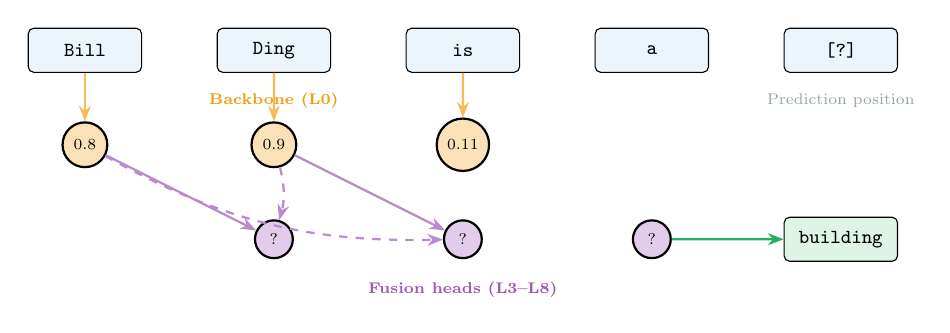
\begin{tikzpicture}[
  scale=0.8, transform shape,
  token/.style={draw, rounded corners=2pt, minimum height=0.7cm, font=\small,
                fill=accent!10, minimum width=1.8cm},
  head/.style={circle, draw, minimum size=0.6cm, font=\scriptsize, thick},
  arr/.style={-{Stealth[length=2mm]}, thick}
]
  % Input tokens
  \node[token] (t1) at (0, 4) {\texttt{Bill}};
  \node[token] (t2) at (3, 4) {\texttt{Ding}};
  \node[token] (t3) at (6, 4) {\texttt{is}};
  \node[token] (t4) at (9, 4) {\texttt{a}};
  \node[token] (t5) at (12, 4) {\texttt{[?]}};

  % Layer 0 - backbone
  \node[head, fill=backbone!30] (h08) at (0, 2.5) {0.8};
  \node[head, fill=backbone!30] (h09) at (3, 2.5) {0.9};
  \node[head, fill=backbone!30] (h011) at (6, 2.5) {0.11};

  % Mid-layer - fusion
  \node[head, fill=fusion!30] (hf1) at (3, 1) {?};
  \node[head, fill=fusion!30] (hf2) at (6, 1) {?};
  \node[head, fill=fusion!30] (hf3) at (9, 1) {?};
  \node[font=\scriptsize\bfseries, fusion] at (6, 0.2) {Fusion heads (L3--L8)};

  % Output
  \node[token, fill=circuit!15] (out) at (12, 1) {\texttt{building}};

  % Connections
  \draw[arr, backbone!70] (t1) -- (h08);
  \draw[arr, backbone!70] (t2) -- (h09);
  \draw[arr, backbone!70] (t3) -- (h011);

  \draw[arr, fusion!70] (h08) -- (hf1);
  \draw[arr, fusion!70] (h09) -- (hf2);
  \draw[arr, fusion!70, dashed] (h08) to[bend right=15] (hf2);
  \draw[arr, fusion!70, dashed] (h09) to[bend left=15] (hf1);

  \draw[arr, circuit] (hf3) -- (out);

  % Labels
  \node[font=\scriptsize\bfseries, backbone] at (3, 3.2) {Backbone (L0)};
  \node[font=\scriptsize, chill] at (12, 3.2) {Prediction position};
\end{tikzpicture}
\end{center}

\vspace{0.3em}
\textbf{Expected:} fusion heads attend \emph{across} the word boundary,\\
composing phonemes from both ``Bill'' and ``Ding'' into ``building.''
\end{frame}

% =============================================
% COMPOUND PUNS
% =============================================
\begin{frame}{Compound puns: chaining operations}

\begin{center}
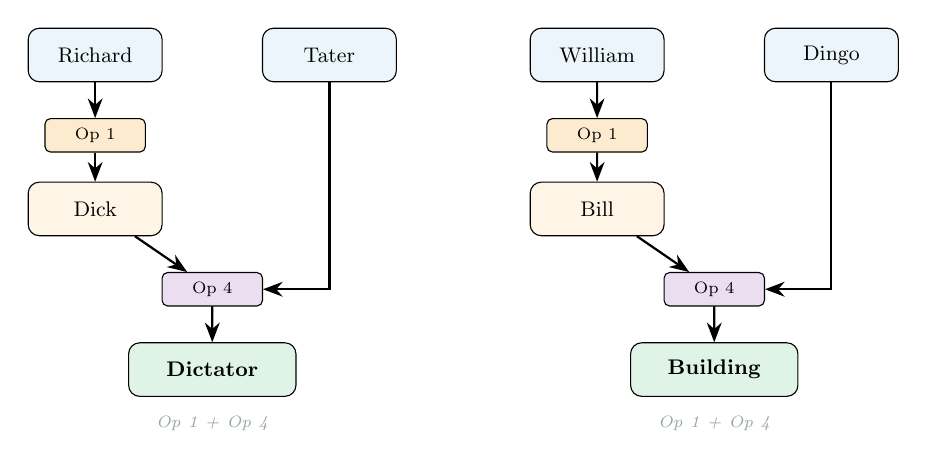
\begin{tikzpicture}[
  scale=0.85, transform shape,
  box/.style={draw, rounded corners=4pt, minimum height=0.8cm, font=\small,
              minimum width=2cm, align=center},
  opbox/.style={draw, rounded corners=2pt, minimum height=0.5cm, font=\scriptsize,
                fill=chill!15, minimum width=1.5cm},
  arr/.style={-{Stealth[length=2.5mm]}, thick}
]
  % Richard Tater -> Dictator
  \node[box, fill=accent!10] (richard) at (0, 2) {Richard};
  \node[box, fill=accent!10] (tater) at (3.5, 2) {Tater};

  \node[opbox, fill=backbone!20] (op1a) at (0, 0.8) {Op 1};
  \node[box, fill=backbone!10] (dick) at (0, -0.3) {Dick};

  \node[opbox, fill=fusion!20] (op4a) at (1.75, -1.5) {Op 4};
  \node[box, fill=circuit!15, minimum width=2.5cm] (dictator) at (1.75, -2.7) {\textbf{Dictator}};

  \draw[arr] (richard) -- (op1a);
  \draw[arr] (op1a) -- (dick);
  \draw[arr] (dick) -- (op4a);
  \draw[arr] (tater) |- (op4a);
  \draw[arr] (op4a) -- (dictator);

  % William Dingo -> Building
  \node[box, fill=accent!10] (william) at (7.5, 2) {William};
  \node[box, fill=accent!10] (dingo) at (11, 2) {Dingo};

  \node[opbox, fill=backbone!20] (op1b) at (7.5, 0.8) {Op 1};
  \node[box, fill=backbone!10] (bill) at (7.5, -0.3) {Bill};

  \node[opbox, fill=fusion!20] (op4b) at (9.25, -1.5) {Op 4};
  \node[box, fill=circuit!15, minimum width=2.5cm] (building) at (9.25, -2.7) {\textbf{Building}};

  \draw[arr] (william) -- (op1b);
  \draw[arr] (op1b) -- (bill);
  \draw[arr] (bill) -- (op4b);
  \draw[arr] (dingo) |- (op4b);
  \draw[arr] (op4b) -- (building);

  % Labels
  \node[font=\scriptsize\itshape, chill] at (1.75, -3.5) {Op 1 + Op 4};
  \node[font=\scriptsize\itshape, chill] at (9.25, -3.5) {Op 1 + Op 4};
\end{tikzpicture}
\end{center}

\vspace{0.3em}
\textbf{Compositionality test:} ablate Op 1 circuit $\Rightarrow$ compound breaks, Op 4 survives.

Ablate Op 4 circuit $\Rightarrow$ compound breaks, Op 1 survives.
\end{frame}

% =============================================
% PART 2 DIVIDER
% =============================================
\begin{frame}[plain,noframenumbering]
\begin{center}
\vfill
  \fcolorbox{black}{white}{\parbox{0.65\textwidth}{\centering\vspace{0.8em}
    {\Large\bfseries Part 2: Methods}
  \vspace{0.8em}}}
\vfill
\end{center}
\end{frame}

% =============================================
% DATASETS
% =============================================
\begin{frame}{Minimal-pair datasets}
\hypertarget{sl:datasets}{}

Each pair follows BLiMP format: \texttt{\{good, bad, target\_token, foil\_token\}}

\vspace{0.5em}
\begin{center}
\small
\begin{tabular}{lll}
\toprule
\textbf{Operation} & \textbf{Good prompt} & \textbf{Target / Foil} \\
\midrule
Op 1 & ``People call Richard by the name'' & Dick / Mark \\
Op 2 & ``Timothy goes by'' & Tim / Tom \\
Op 3 & ``The letter J is pronounced'' & Jay / Gee \\
Op 4 & ``Bill Ding sounds like'' & building / nothing \\
Op 5 & ``Neil sounds like'' & kneel / wheel \\
Op 7 & ``Mike Rowave sounds like'' & microwave / nothing \\
\bottomrule
\end{tabular}
\end{center}

\vspace{0.5em}
\textbf{Evaluation:} logit difference at final position.

\textbf{Gate:} $>$70\% accuracy before circuit discovery.

\vspace{0.5em}
Ops 2, 3, 5 are procedurally expandable (CMU Dict).\\
Ops 1, 4, 7 are controlled vocabularies.
\end{frame}

% =============================================
% TOKENIZATION AUDIT
% =============================================
\begin{frame}{Tokenization audit}

BPE tokenization can break phonological tasks:

\vspace{0.5em}
\begin{center}
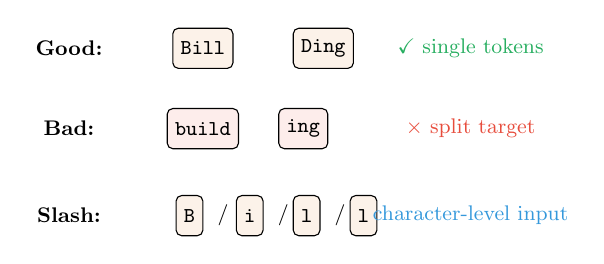
\begin{tikzpicture}[
  scale=0.85, transform shape,
  tok/.style={draw, rounded corners=2pt, minimum height=0.6cm, font=\ttfamily\small,
              fill=tok!10},
  bad/.style={draw, rounded corners=2pt, minimum height=0.6cm, font=\ttfamily\small,
              fill=phoneme!10}
]
  % Good tokenization
  \node[font=\small\bfseries] at (-2, 1) {Good:};
  \node[tok] (g1) at (0, 1) {Bill};
  \node[tok] (g2) at (1.8, 1) {Ding};
  \node[font=\small, circuit] at (4, 1) {$\checkmark$ single tokens};

  % Bad tokenization
  \node[font=\small\bfseries] at (-2, -0.2) {Bad:};
  \node[bad] (b1) at (0, -0.2) {build};
  \node[bad] (b2) at (1.5, -0.2) {ing};
  \node[font=\small, phoneme] at (4, -0.2) {$\times$ split target};

  % Slash condition
  \node[font=\small\bfseries] at (-2, -1.5) {Slash:};
  \node[tok] (s1) at (-0.2, -1.5) {B};
  \node[font=\small] at (0.3, -1.5) {/};
  \node[tok] (s2) at (0.7, -1.5) {i};
  \node[font=\small] at (1.2, -1.5) {/};
  \node[tok] (s3) at (1.55, -1.5) {l};
  \node[font=\small] at (2.05, -1.5) {/};
  \node[tok] (s4) at (2.4, -1.5) {l};
  \node[font=\small, accent] at (4, -1.5) {character-level input};
\end{tikzpicture}
\end{center}

\vspace{0.5em}
Following \href{https://aclanthology.org/2026.latechclfl-1.9}{Liao \& Shi (2026)}: if slash-delimited input improves Op 4 accuracy, the circuit \emph{exists} but is bottlenecked by tokenization.

\vspace{0.5em}
$\Rightarrow$ Weight-space capacity vs.\ activation-flow distinction.
\end{frame}

% =============================================
% CIRCUIT DISCOVERY
% =============================================
\begin{frame}{Three discovery methods}
\hypertarget{sl:discovery}{}

\begin{center}
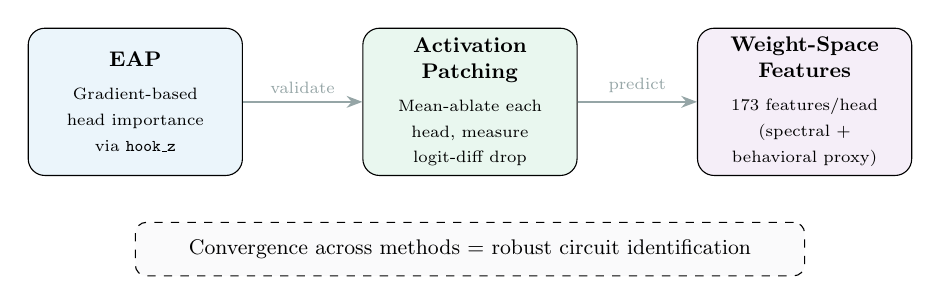
\begin{tikzpicture}[
  scale=0.85, transform shape,
  method/.style={draw, rounded corners=6pt, minimum height=2.2cm, minimum width=3.2cm,
                 align=center, font=\small},
  arr/.style={-{Stealth[length=2mm]}, thick, chill}
]
  \node[method, fill=accent!10] (eap) at (0, 0) {
    \textbf{EAP}\\[3pt]
    {\scriptsize Gradient-based}\\
    {\scriptsize head importance}\\
    {\scriptsize via \texttt{hook\_z}}
  };

  \node[method, fill=circuit!10] (ap) at (5, 0) {
    \textbf{Activation}\\
    \textbf{Patching}\\[3pt]
    {\scriptsize Mean-ablate each}\\
    {\scriptsize head, measure}\\
    {\scriptsize logit-diff drop}
  };

  \node[method, fill=fusion!10] (ws) at (10, 0) {
    \textbf{Weight-Space}\\
    \textbf{Features}\\[3pt]
    {\scriptsize 173 features/head}\\
    {\scriptsize (spectral +}\\
    {\scriptsize behavioral proxy)}
  };

  \draw[arr] (eap) -- (ap) node[midway, above, font=\scriptsize] {validate};
  \draw[arr] (ap) -- (ws) node[midway, above, font=\scriptsize] {predict};

  \node[draw, dashed, rounded corners=4pt, fill=chill!5, minimum width=10cm,
        minimum height=0.8cm, font=\small] at (5, -2.2) {
    Convergence across methods $=$ robust circuit identification
  };
\end{tikzpicture}
\end{center}
\end{frame}

% =============================================
% PART 3 DIVIDER
% =============================================
\begin{frame}[plain,noframenumbering]
\begin{center}
\vfill
  \fcolorbox{black}{white}{\parbox{0.65\textwidth}{\centering\vspace{0.8em}
    {\Large\bfseries Part 3: Circuits}
  \vspace{0.8em}}}
\vfill
\end{center}
\end{frame}

% =============================================
% BACKBONE HYPOTHESIS
% =============================================
\begin{frame}{The backbone hypothesis}
\hypertarget{sl:backbone}{}

Prior finding: heads L0H8, L0H9, L0H11 participate in \emph{every} known circuit (IOI, SVA, greater-than, induction).

\vspace{0.5em}
\begin{center}
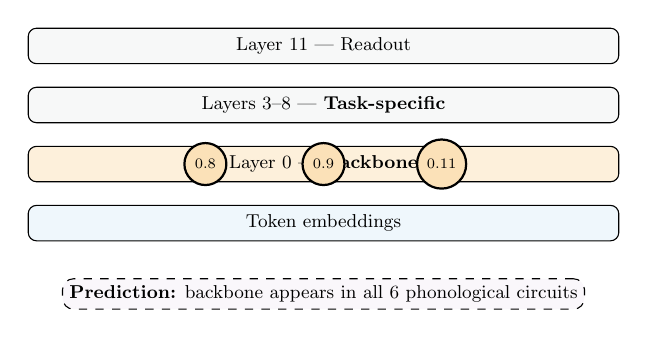
\begin{tikzpicture}[
  scale=0.75, transform shape,
  layer/.style={draw, rounded corners=3pt, minimum height=0.6cm, font=\small,
                minimum width=10cm, fill=chill!8},
  head/.style={circle, draw, minimum size=0.55cm, font=\scriptsize, thick}
]
  % Layers
  \node[layer] (l11) at (0, 4) {Layer 11 --- Readout};
  \node[layer] (l8) at (0, 3) {Layers 3--8 --- \textbf{Task-specific}};
  \node[layer, fill=backbone!15] (l0) at (0, 2) {Layer 0 --- \textbf{Backbone}};
  \node[layer, fill=accent!8] (emb) at (0, 1) {Token embeddings};

  % Backbone heads
  \node[head, fill=backbone!30] at (-2, 2) {0.8};
  \node[head, fill=backbone!30] at (0, 2) {0.9};
  \node[head, fill=backbone!30] at (2, 2) {0.11};

  % Question
  \node[draw, dashed, rounded corners=4pt, fill=fusion!5, font=\small,
        minimum width=8cm] at (0, -0.2) {
    \textbf{Prediction:} backbone appears in all 6 phonological circuits
  };
\end{tikzpicture}
\end{center}

\vspace{0.3em}
If confirmed: the ``operating system'' extends to phonological computation.
\end{frame}

% =============================================
% FUSION HEADS
% =============================================
\begin{frame}{Predicted circuit architectures}
\hypertarget{sl:fusionheads}{}

\begin{center}
\small
\begin{tabular}{llll}
\toprule
\textbf{Op} & \textbf{Expected circuit type} & \textbf{Key heads} & \textbf{Analogy} \\
\midrule
1 & Associative lookup & Mid-layer OV & Name-mover (IOI) \\
2 & Positional truncation & Positional attn & Acronym circuit \\
3 & G2P map & Letter $\to$ phoneme & Letter-mover \\
\rowcolor{fusion!8}
4 & \textbf{Cross-boundary fusion} & \textbf{Novel L3--L8} & \textbf{None known} \\
5 & Phoneme identity & Mid-layer probe & Rhyme probes \\
7 & Reverse decomposition & Creative gen & Expected to fail \\
\bottomrule
\end{tabular}
\end{center}

\vspace{0.8em}
Op 4 is the core novel finding: if cross-boundary fusion heads exist,\\
they are \textbf{a new circuit type} not identified in any prior work.
\end{frame}

% =============================================
% OVERLAP MATRIX
% =============================================
\begin{frame}{Circuit overlap matrix}

\begin{center}
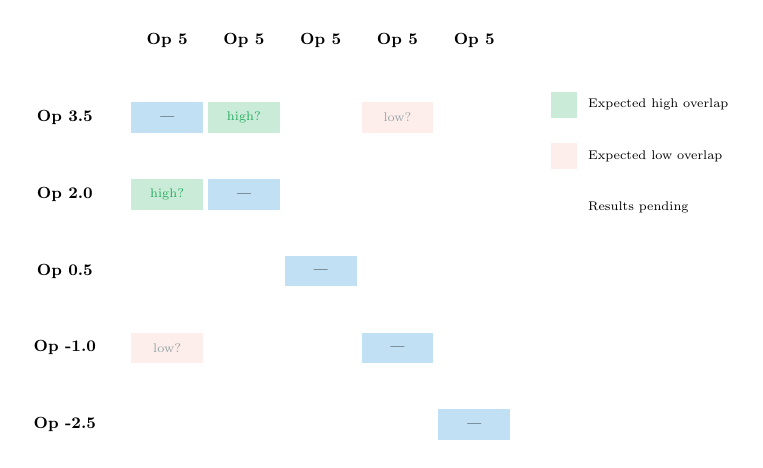
\begin{tikzpicture}[scale=0.65, transform shape]
  % Matrix
  \def\ops{{"1","2","3","4","5"}}

  % Headers
  \foreach \i in {0,...,4} {
    \pgfmathparse{\ops[\i]}
    \node[font=\small\bfseries] at (\i*1.5 + 1.5, 5) {Op \pgfmathresult};
    \node[font=\small\bfseries] at (-0.5, 3.5 - \i*1.5) {Op \pgfmathresult};
  }

  % Diagonal
  \foreach \i in {0,...,4} {
    \fill[accent!30] (\i*1.5 + 0.8, 3.8 - \i*1.5) rectangle (\i*1.5 + 2.2, 3.2 - \i*1.5);
    \node[font=\scriptsize] at (\i*1.5 + 1.5, 3.5 - \i*1.5) {---};
  }

  % Expected high overlap (1-2: both name shortening)
  \fill[circuit!25] (0.8 + 1.5, 3.8 - 0) rectangle (2.2 + 1.5, 3.2 - 0);
  \node[font=\scriptsize, circuit] at (1.5 + 1.5, 3.5) {high?};
  \fill[circuit!25] (0.8, 3.8 - 1.5) rectangle (2.2, 3.2 - 1.5);
  \node[font=\scriptsize, circuit] at (1.5, 2.0) {high?};

  % Expected low overlap (4 vs others)
  \fill[phoneme!10] (0.8 + 4.5, 3.8 - 0) rectangle (2.2 + 4.5, 3.2 - 0);
  \node[font=\scriptsize, chill] at (1.5 + 4.5, 3.5) {low?};
  \fill[phoneme!10] (0.8, 3.8 - 4.5) rectangle (2.2, 3.2 - 4.5);
  \node[font=\scriptsize, chill] at (1.5, -1.0) {low?};

  % Fill rest with ?
  \foreach \i in {0,...,4} {
    \foreach \j in {0,...,4} {
      \pgfmathtruncatemacro{\test}{\i == \j ? 1 : 0}
      \ifnum\test=0
        % Only fill if not already filled
      \fi
    }
  }

  % Legend
  \fill[circuit!25] (9, 3.5) rectangle (9.5, 4);
  \node[font=\scriptsize, right] at (9.6, 3.75) {Expected high overlap};
  \fill[phoneme!10] (9, 2.5) rectangle (9.5, 3);
  \node[font=\scriptsize, right] at (9.6, 2.75) {Expected low overlap};
  \node[font=\scriptsize, right] at (9.6, 1.75) {Results pending};
\end{tikzpicture}
\end{center}

\vspace{0.3em}
If Op 4 uses \emph{unique} heads not shared with any other operation:\\
evidence for specialized phonological circuitry.
\end{frame}

% =============================================
% COMPOSITION
% =============================================
\begin{frame}{Compositional validation protocol}
\hypertarget{sl:composition}{}

\begin{center}
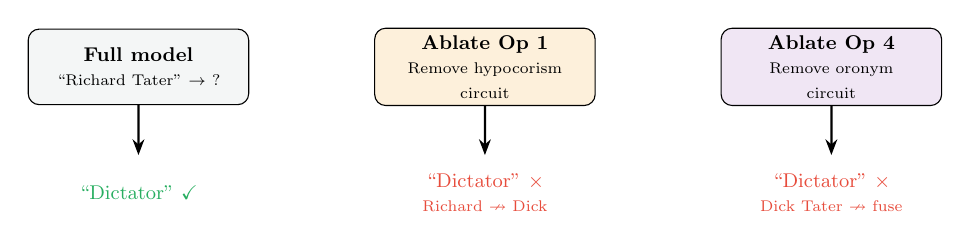
\begin{tikzpicture}[
  scale=0.8, transform shape,
  test/.style={draw, rounded corners=4pt, minimum height=1.2cm, minimum width=3.5cm,
               align=center, font=\small},
  result/.style={font=\small, align=center},
  arr/.style={-{Stealth[length=2mm]}, thick}
]
  % Tests
  \node[test, fill=chill!10] (full) at (0, 2) {
    \textbf{Full model}\\
    {\scriptsize ``Richard Tater'' $\to$ ?}
  };

  \node[test, fill=backbone!15] (abl1) at (5.5, 2) {
    \textbf{Ablate Op 1}\\
    {\scriptsize Remove hypocorism}\\
    {\scriptsize circuit}
  };

  \node[test, fill=fusion!15] (abl4) at (11, 2) {
    \textbf{Ablate Op 4}\\
    {\scriptsize Remove oronym}\\
    {\scriptsize circuit}
  };

  % Expected results
  \node[result, circuit] at (0, 0) {``Dictator'' $\checkmark$};
  \node[result, phoneme] at (5.5, 0) {``Dictator'' $\times$\\{\scriptsize Richard $\nrightarrow$ Dick}};
  \node[result, phoneme] at (11, 0) {``Dictator'' $\times$\\{\scriptsize Dick Tater $\nrightarrow$ fuse}};

  \draw[arr] (full) -- (0, 0.6);
  \draw[arr] (abl1) -- (5.5, 0.6);
  \draw[arr] (abl4) -- (11, 0.6);
\end{tikzpicture}
\end{center}

\vspace{0.5em}
Each component circuit is \textbf{independently necessary}.

$\Rightarrow$ True compositional structure, not a single monolithic circuit.
\end{frame}

% =============================================
% PART 4 DIVIDER
% =============================================
\begin{frame}[plain,noframenumbering]
\begin{center}
\vfill
  \fcolorbox{black}{white}{\parbox{0.65\textwidth}{\centering\vspace{0.8em}
    {\Large\bfseries Part 4: Implications}
  \vspace{0.8em}}}
\vfill
\end{center}
\end{frame}

% =============================================
% TOKENIZATION BOTTLENECK
% =============================================
\begin{frame}{Tokenization as computational bottleneck}
\hypertarget{sl:tokenization}{}

\begin{center}
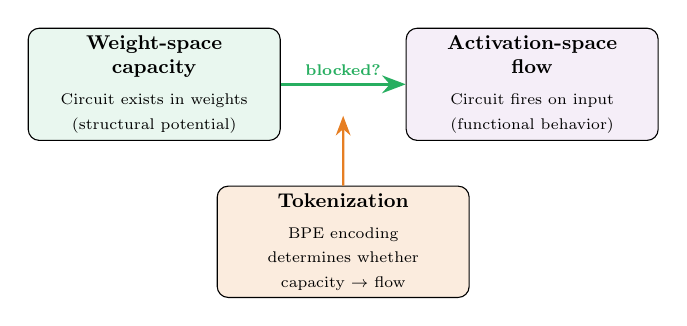
\begin{tikzpicture}[
  scale=0.8, transform shape,
  box/.style={draw, rounded corners=4pt, minimum height=1.5cm, minimum width=4cm,
              align=center, font=\small}
]
  \node[box, fill=circuit!10] (capacity) at (0, 0) {
    \textbf{Weight-space}\\
    \textbf{capacity}\\[3pt]
    {\scriptsize Circuit exists in weights}\\
    {\scriptsize (structural potential)}
  };

  \node[box, fill=fusion!10] (flow) at (6, 0) {
    \textbf{Activation-space}\\
    \textbf{flow}\\[3pt]
    {\scriptsize Circuit fires on input}\\
    {\scriptsize (functional behavior)}
  };

  \node[box, fill=tok!15] (bottleneck) at (3, -2.5) {
    \textbf{Tokenization}\\[3pt]
    {\scriptsize BPE encoding}\\
    {\scriptsize determines whether}\\
    {\scriptsize capacity $\to$ flow}
  };

  \draw[-{Stealth[length=3mm]}, very thick, circuit] (capacity) -- (flow)
    node[midway, above, font=\scriptsize\bfseries] {blocked?};
  \draw[-{Stealth[length=2.5mm]}, thick, tok] (bottleneck) -- (3, -0.5);
\end{tikzpicture}
\end{center}

\vspace{0.3em}
If Op 4 accuracy improves with character-level input (slash condition),\\
GPT-2 \emph{has} the circuit but BPE \emph{prevents it from firing}.
\end{frame}

% =============================================
% DISCUSSION
% =============================================
\begin{frame}{What this tells us}
\hypertarget{sl:discussion}{}

\textbf{If the oronym circuit exists:}
\begin{itemize}
  \item GPT-2 learned cross-boundary phonological assembly from orthographic training alone
  \item Phonological computation is not a single undifferentiated capability --- distinct operations use distinct circuits
  \item The backbone ``operating system'' extends to phonology
\end{itemize}

\vspace{0.8em}
\textbf{If it doesn't:}
\begin{itemize}
  \item Behavioral phonological performance (probes, PhonologyBench) may be statistical co-occurrence, not structured computation
  \item The weight-capacity vs.\ activation-flow gap is real and measurable
\end{itemize}

\vspace{0.8em}
Either outcome is a publishable finding.
\end{frame}

% =============================================
% EXAMPLES
% =============================================
\begin{frame}{The dataset: selected examples}

\begin{center}
\small
\begin{tabular}{lll}
\toprule
\textbf{Input} & \textbf{Target} & \textbf{Operation chain} \\
\midrule
Richard Tater & Dictator & Op 1 + Op 4 \\
William Ding & Building & Op 1 + Op 4 \\
Elizabeth Aardvark & Lizard & Op 2 + Op 4 \\
\midrule
Bill Ding & Building & Op 4 only \\
Curt Ain & Curtain & Op 4 only \\
Brock Lee & Broccoli & Op 4 only \\
Barb Dwyer & Barbed wire & Op 4 only \\
\midrule
Mike Rowave & Microwave & Op 7 (reverse) \\
Dan Druff & Dandruff & Op 4 only \\
Herb Ivore & Herbivore & Op 4 only \\
\bottomrule
\end{tabular}
\end{center}

\vspace{0.5em}
99 oronym pairs, 32 hypocorism pairs, 120 homophone pairs.

446 total minimal pairs across 6 operations.
\end{frame}

% =============================================
% STATUS
% =============================================
\begin{frame}{Current status}

\begin{center}
\small
\begin{tabular}{lll}
\toprule
\textbf{Component} & \textbf{Status} & \textbf{Next step} \\
\midrule
Paper outline & Complete & --- \\
6 operation definitions & Complete & --- \\
Minimal-pair datasets & Designed & Build \& audit tokenization \\
Behavioral validation & Pending & Run on GPT-2 S/M/L \\
EAP discovery & Pending & Run per-operation \\
Activation patching & Pending & Validate EAP rankings \\
Weight-space prediction & Pending & Cross-reference \\
Compositional ablation & Pending & After circuit ID \\
Tokenization experiment & Pending & Slash-condition test \\
\bottomrule
\end{tabular}
\end{center}

\vspace{0.8em}
Target venue: COLM, Findings of ACL, or MI workshop.
\end{frame}

% =============================================
% THANK YOU
% =============================================
\begin{frame}{Thank you}

\begin{center}
\vfill
{\Large Phonological Assembly Circuits in GPT-2}

\vspace{1.5em}

\textbf{Repository:} \href{https://github.com/elliottower/phonetic-circuits}{\texttt{github.com/elliottower/phonetic-circuits}}

\textbf{Contact:} \texttt{elliot@elliottower.ai}

\vspace{1.5em}

\rule{0.3\textwidth}{0.2pt}

\vspace{1em}

{\small \textit{``Bill Ding'' $\to$ ``building''}}

\vfill
\end{center}
\end{frame}

\end{document}
